%----------------------------------------------------------------------------
\chapter{Sakkszabályok és tündérsakk}\label{chap:rules}
%----------------------------------------------------------------------------

\section{A FIDE-szabályok motor szempontjából fontos részei}

A motor a Nemzetközi Sakkszövetség (FIDE) hivatalos szabályzatát~\cite{FIDELaws} valósítja meg. A játék $8\times8$-as táblán, két fél között zajlik. Mindkét fél 16 bábuval indul: király, vezér, két bástya, két futó, két huszár és nyolc gyalog. A szabályok közül a következők igényelnek a lépésgenerátorban külön kezelést:

\begin{itemize}
	\item \emph{Csúszó bábuk:} a bástya vízszintesen és függőlegesen, a futó átlósan, a vezér mindkét módon léphet tetszőleges távolságra, de nem ugorhat át más bábut.
	\item \emph{Ugró bábu:} a huszár ,,L'' alakban lép, és átugorhatja a köztes mezőket.
	\item \emph{Gyalog:} előre egyet, kiinduló sorából kettőt léphet, átlósan üt. Ha a hetedik (sötét esetén a második) sorról az utolsó sorra lép, átváltozik huszárrá, futóvá, bástyává vagy vezérré.
	\item \emph{En passant:} ha a gyalog kettőt lép, és ezzel egy ellenfél gyalog mellé érkezik, az ellenfél a következő lépésben úgy ütheti, mintha csak egyet lépett volna.
	\item \emph{Sáncolás:} a király két mezőt lép a bástya felé, a bástya átugrik mellé. Feltétele, hogy egyik bábu se lépett még, köztük ne álljon bábu, és a király se sakkban ne álljon, se megtámadott mezőn ne haladjon át, se ilyenre ne érkezzen.
	\item \emph{Sakk, matt, patt:} szabálytalan minden lépés, amely után a lépő fél királya támadás alatt marad. Ha a lépésre következő félnek nincs szabályos lépése, a játszma sakkban matttal, egyébként pattal (döntetlen) ér véget.
	\item \emph{Döntetlen szabályok:} a háromszori állásismétlés, az ötvenlépéses szabály (50 lépés ütés és gyaloglépés nélkül), valamint az elégtelen anyag (pl. király és futó a király ellen), amellyel matt nem adható.
\end{itemize}

A versenyjátszmákban a gondolkodási időt sakkóra méri. A motor a két legelterjedtebb módot támogatja: a fix lépésenkénti időt és az időbeosztást, ahol mindkét fél alapidővel indul, és minden lépés után bónuszidőt kap.

\section{A tündérsakk alapelvei}

A tündérsakk gyűjtőfogalom: minden olyan változatot ide sorolunk, amely nem szabványos bábukat, táblát vagy szabályokat használ~\cite{Pritchard07}. A tündérbábuk mozgását általában a hagyományos bábuk alapmozgásaiból, más néven atomokból rakják össze. Ralph Betza jelölésrendszerében~\cite{Betza} például \texttt{W} a vízszintes/függőleges egylépéses, \texttt{F} az átlós egylépéses, \texttt{N} a huszárugrás; a betű megduplázása (\texttt{WW}, \texttt{FF}) vagy a \texttt{R}, \texttt{B} jelek a csúszó, tetszőleges távolságú változatot jelölik. Ebben a rendszerben a vezér \texttt{Q = RB}, a huszár \texttt{N}.

Az összetett bábuk két vagy több atom unióját mozgatják. A legismertebbek:
\begin{itemize}
	\item {Arkangyal} (BN): futó + huszár,
	\item {Kancellár} (RN): bástya + huszár,
	\item {Amazon} (QN): vezér + huszár.
\end{itemize}

\begin{figure}[!ht]
	\centering
	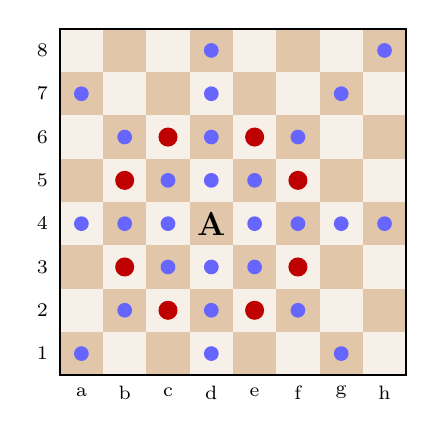
\begin{tikzpicture}[scale=0.55]
		\foreach \x in {0,...,7} \foreach \y in {0,...,7} {
			\pgfmathparse{mod(\x+\y,2)==0 ? "brown!45" : "brown!12"}
			\fill[\pgfmathresult] (\x,\y) rectangle ++(1,1);
		}
		\foreach \dx/\dy in {1/0,-1/0,0/1,0/-1,1/1,1/-1,-1/1,-1/-1} {
			\foreach \k in {1,...,7} {
				\pgfmathsetmacro{\px}{3+\k*\dx}\pgfmathsetmacro{\py}{3+\k*\dy}
				\ifdim \px pt>-1pt \ifdim \px pt<8pt \ifdim \py pt>-1pt \ifdim \py pt<8pt
					\fill[blue!60] (\px+0.5,\py+0.5) circle (0.17);
				\fi\fi\fi\fi
			}
		}
		\foreach \dx/\dy in {1/2,2/1,-1/2,-2/1,1/-2,2/-1,-1/-2,-2/-1} {
			\fill[red!75!black] (3+\dx+0.5,3+\dy+0.5) circle (0.22);
		}
		\node[font=\bfseries\large] at (3.5,3.5) {A};
		\draw[thick] (0,0) rectangle (8,8);
		\foreach \f [count=\i from 0] in {a,...,h} \node[font=\scriptsize] at (\i+0.5,-0.4) {\f};
		\foreach \r in {1,...,8} \node[font=\scriptsize] at (-0.4,\r-0.5) {\r};
	\end{tikzpicture}
	\caption{Az Amazon lépései a d4 mezőről: kék a vezérszerű , piros a huszárszerű célmezők.}
	\label{fig:amazonMoves}
\end{figure}

Az Amazon (\ref{fig:amazonMoves}.~ábra) üres táblán egy középső mezőről akár 35 mezőt is elérhet (27 vezérszerű + 8 huszárugrás), szemben a vezér 27 mezőjével. A huszárugrás az egyetlen olyan támadási forma, amelyet a vezér nem tud kivédeni közbeállással, ezért az Amazon egyedül is mattot adhat a magára hagyott királynak. Mivel a király ilyen bábu ellen különösen sebezhető, az Amazon jelentősen felülmúlja a vezért; a szakirodalom értékét általában 12--13 gyalogegységre teszi~\cite{ChessVariantsAmazon}. A motorban az Amazon a vezér helyén áll, és az ilyen változatban a vezér teljesen eltűnik a játékból: a gyalog is Amazonná változik a vezér helyett.
